\documentclass[10pt]{article}
\usepackage[margin=0.52in]{geometry}
\usepackage{amsmath,amssymb,booktabs,graphicx,float,microtype}
\usepackage[T1]{fontenc}
\setlength{\parindent}{0pt}
\setlength{\parskip}{3pt}
\newcommand{\ket}[1]{\lvert #1\rangle}
\begin{document}
\begin{center}
{\Large\bfseries Experiment 06: end-to-end ECD state preparation}\\[-1pt]
{\small Five state representations, exact common scoring, and saved circuits}
\end{center}

\textbf{Question and test case.}
Starting from qubit ground state and oscillator vacuum,
$\ket{0}_q\ket{0}_o$, we optimize an echoed conditional displacement
(ECD)-plus-qubit-rotation circuit to prepare
the oscillator target
\[
 \ket{\psi_{\rm target}}=(\ket9+\ket{10})/\sqrt2 .
\]
Here $\ket m$ means exactly $m$ oscillator photons.  ``Layers'' means the
number $n\in\{4,8,12,16,20\}$ of ECD-plus-rotation blocks.  A saved layer is
$[\beta,\phi,\theta,\gamma]$: $\beta$ is complex, the angles are in radians,
$\gamma=0$, and the two ECD branches are displaced by $-\beta/2$ and
$+\beta/2$.  Every method has three deterministic restarts. Adam is an adaptive
gradient optimizer. Depths 4--16 use 1,200 Adam updates per restart; depth 20
uses 10,000 because shorter runs can
stop before a late breakthrough. Thus methods are budget-matched at fixed
depth, but the 16-to-20 change is not a depth-only comparison.

\textbf{The five methods.}
Full coherent paths retains all $2^n$ analytic paths and has no oscillator
cutoff. The Fock basis is the photon-number basis $\ket0,\ket1,\ldots$.
Analytic Fock propagates two 48-entry vectors, covering photon numbers 0--47,
using
\[
 D(a)\ket0=\ket a,\qquad
 D(a)\ket k=(\hat a^\dagger-a^*)D(a)\ket{k-1}/\sqrt{k}.
\]
Dense numerical Fock instead truncates $a$ first and materializes
$D_{48}^{\rm num}(a)=\exp(a a_{48}^\dagger-a^*a_{48})$ and every $96\times96$
joint layer unitary. It is unitary inside the grid but has a different boundary;
matrix exponentials and state propagation use complex64, while exact rescoring
uses float64.
Continuous anchors and squeezed packets retain 32 packets in each qubit branch
plus two 48-entry working arrays (160 complex coefficients between layers;
224 just before compression). When a branch exceeds 32 candidates, residual pivots seed movable
centers, 12 inner Adam steps optimize the centers, and a global least-squares
solve refits coefficients.  Squeezed packets add 16 steps for one bounded
complex squeeze per packet.  Their forward pass uses the compressed state;
their outer gradient uses the heuristic straight-through derivative of the
projection.  Thus internal approximate scores are never used to select a
winner.

\textbf{Exact common score.}
Writing the exact output as
$\ket\Psi=\sum_q\ket q\sum_jc_{qj}\ket{z_{qj}}$ and using
$\langle m\vert z\rangle=e^{-|z|^2/2}z^m/\sqrt{m!}$, every restart is ranked by
\[
 F=\sum_{q=0}^1\left|\sum_jc_{qj}e^{-|z_{qj}|^2/2}
 \frac{z_{qj}^9/\sqrt{9!}+z_{qj}^{10}/\sqrt{10!}}{\sqrt2}\right|^2 .
\]
This is the fidelity after tracing out the qubit and has no Fock cutoff.
A separate 96-level conversion agrees within $7.1\times10^{-13}$.

\begin{table}[H]
\centering\scriptsize
\setlength{\tabcolsep}{3.5pt}
\begin{tabular}{r l r r r}
\toprule
$n$ & optimizer & exact $F$ & $1-F$ & all-restart wall time (s)\\
\midrule
4 & full coherent & .505018513 & .494981487 & 2.50\\
  & analytic Fock & .505018513 & .494981487 & 3.74\\
  & dense numerical Fock & .505018552 & .494981448 & 17.44\\
  & squeezed packets & .505018513 & .494981487 & 4.24\\
  & continuous anchors & .505018513 & .494981487 & 5.04\\
\midrule
8 & full coherent & .857536427 & .142463573 & 5.87\\
  & analytic Fock & .857534952 & .142465048 & 7.21\\
  & dense numerical Fock & .857536425 & .142463575 & 33.35\\
  & squeezed packets & .857534965 & .142465035 & 114.67\\
  & continuous anchors & .857534973 & .142465027 & 63.75\\
\midrule
12 & full coherent & .974346473 & .025653527 & 14.53\\
   & analytic Fock & .974350445 & .025649555 & 10.87\\
   & dense numerical Fock & .974345335 & .025654665 & 56.51\\
   & squeezed packets & .974348265 & .025651735 & 360.45\\
   & continuous anchors & .974351803 & .025648197 & 180.37\\
\midrule
16 & full coherent & \textbf{.988280951} & \textbf{.011719049} & 36.70\\
   & analytic Fock & .986552032 & .013447968 & \textbf{14.77}\\
   & dense numerical Fock & .988280877 & .011719123 & 77.49\\
   & squeezed packets & .987050831 & .012949169 & 659.39\\
   & continuous anchors & .987752877 & .012247123 & 297.66\\
\midrule
20 & full coherent & \textbf{.998767876} & \textbf{.001232124} & 2038.69\\
   & analytic Fock & .998767507 & .001232493 & \textbf{53.22}\\
   & dense numerical Fock & .998767867 & .001232133 & 483.39\\
   & squeezed packets & .998764935 & .001235065 & 4703.63\\
   & continuous anchors & .998764050 & .001235950 & 2959.72\\
\bottomrule
\end{tabular}
\caption{The winner at each method/depth is the restart with largest exact
$F$. Wall time includes all three restarts, first compilation, and exact host
rescoring. The step
budget is 1,200 for $n\leq16$ and 10,000 for $n=20$. At $n=4$ there is no
compression because each branch has only eight paths.}
\end{table}

\newpage
\textbf{Search cost, accuracy, and physical gate time.}
Optimization wall time is computer search time.  Gate time estimates how long
the saved circuit would run on hardware.  The Coherax convention is
\[
T_C=\sum_i\left[24\,{\rm ns}+\max\left(
\frac{|\beta_i|}{(2\pi\,50\,{\rm kHz})20},48\,{\rm ns}\right)\right].
\]
The repository cannot compile new arbitrary sequences with the upstream
Eickbusch pulse compiler.  We therefore report, and label as a lower bound,
\[
T_{E,{\rm LB}}=\sum_i\max\left(
\frac{|\beta_i|}{(2\pi\,33\,{\rm kHz})30},224\,{\rm ns}\right),
\]
where 224 ns is two 24 ns qubit pulses plus four 44 ns displacement pulses.
It is not a compiled waveform duration.

\begin{figure}[H]
\centering
\begin{minipage}{.49\linewidth}\centering
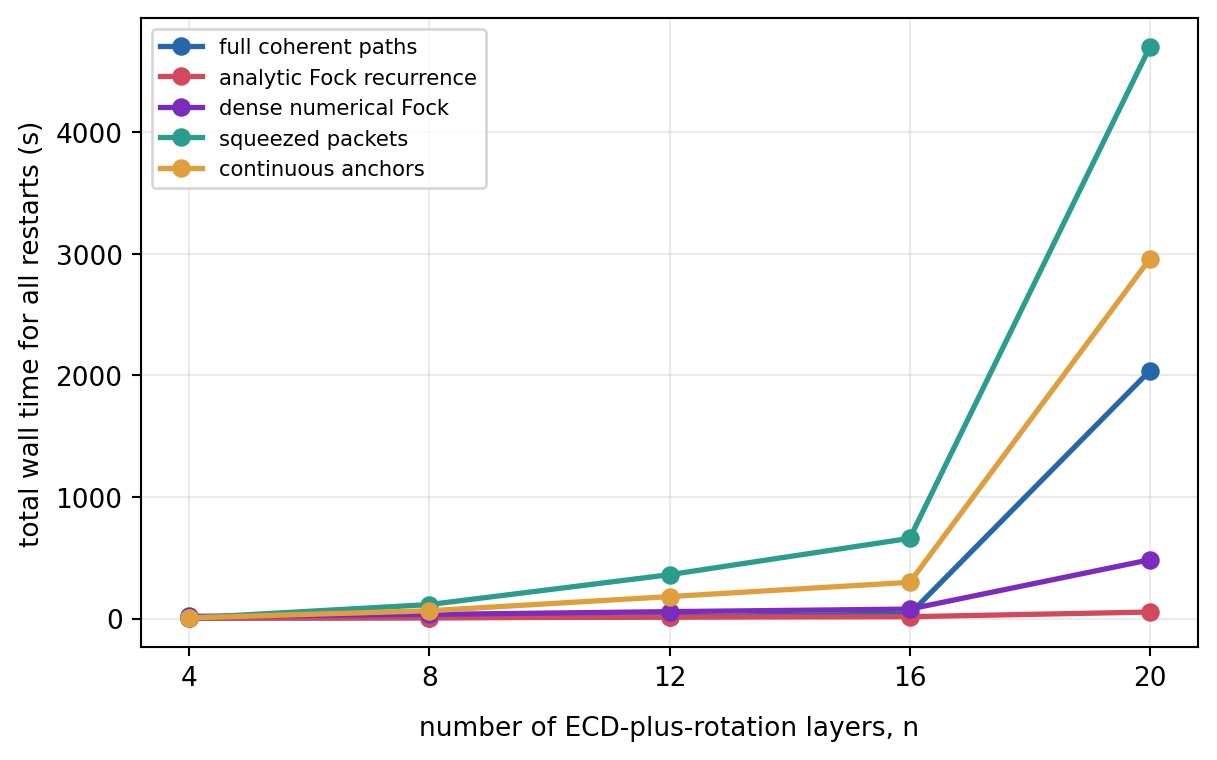
\includegraphics[width=\linewidth]{figs/wall_time_vs_layers.png}
\end{minipage}\hfill
\begin{minipage}{.49\linewidth}\centering
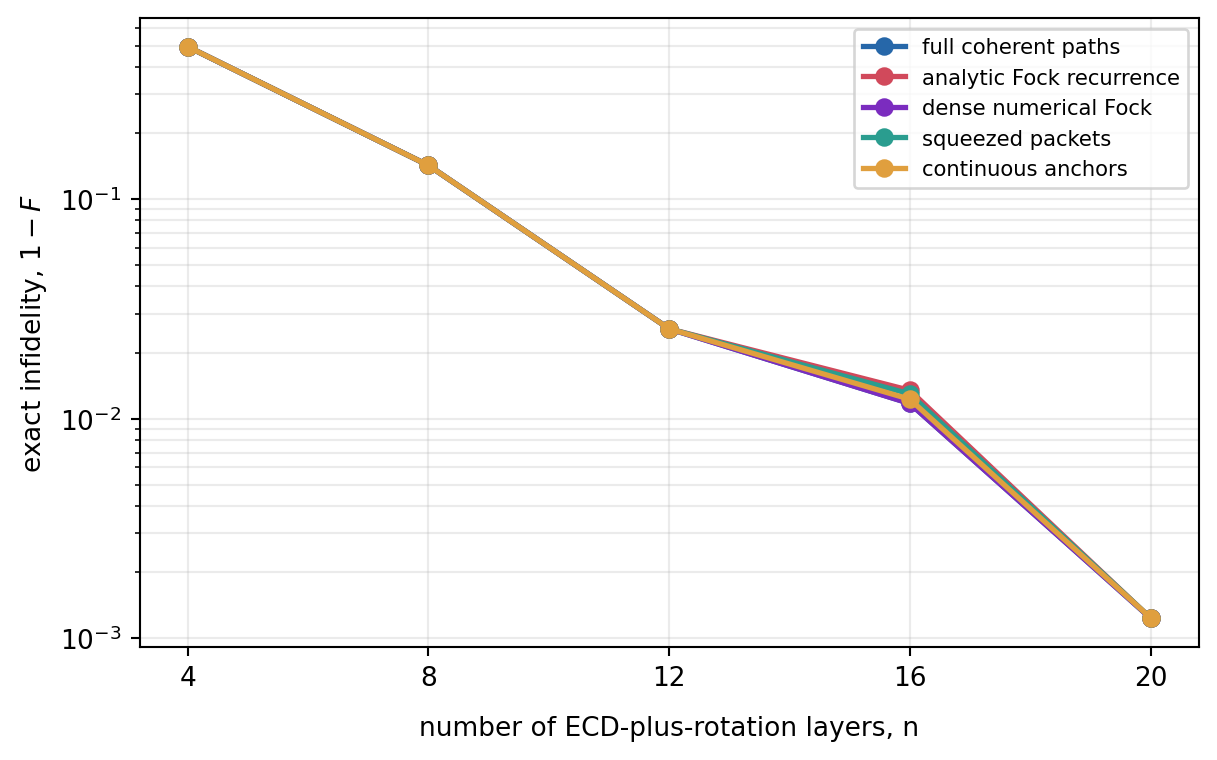
\includegraphics[width=\linewidth]{figs/infidelity_vs_layers.png}
\end{minipage}

\vspace{3pt}
\begin{minipage}{.49\linewidth}\centering
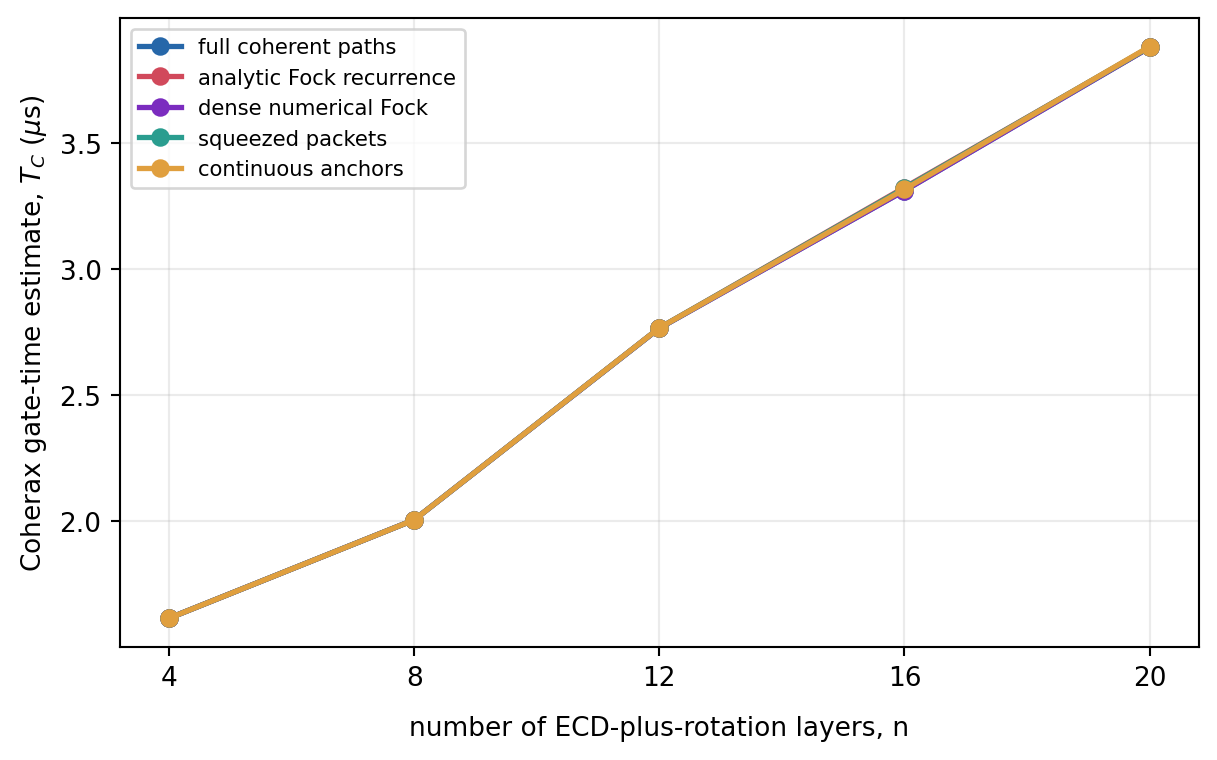
\includegraphics[width=\linewidth]{figs/gate_time_coherax_vs_layers.png}
\end{minipage}\hfill
\begin{minipage}{.49\linewidth}\centering
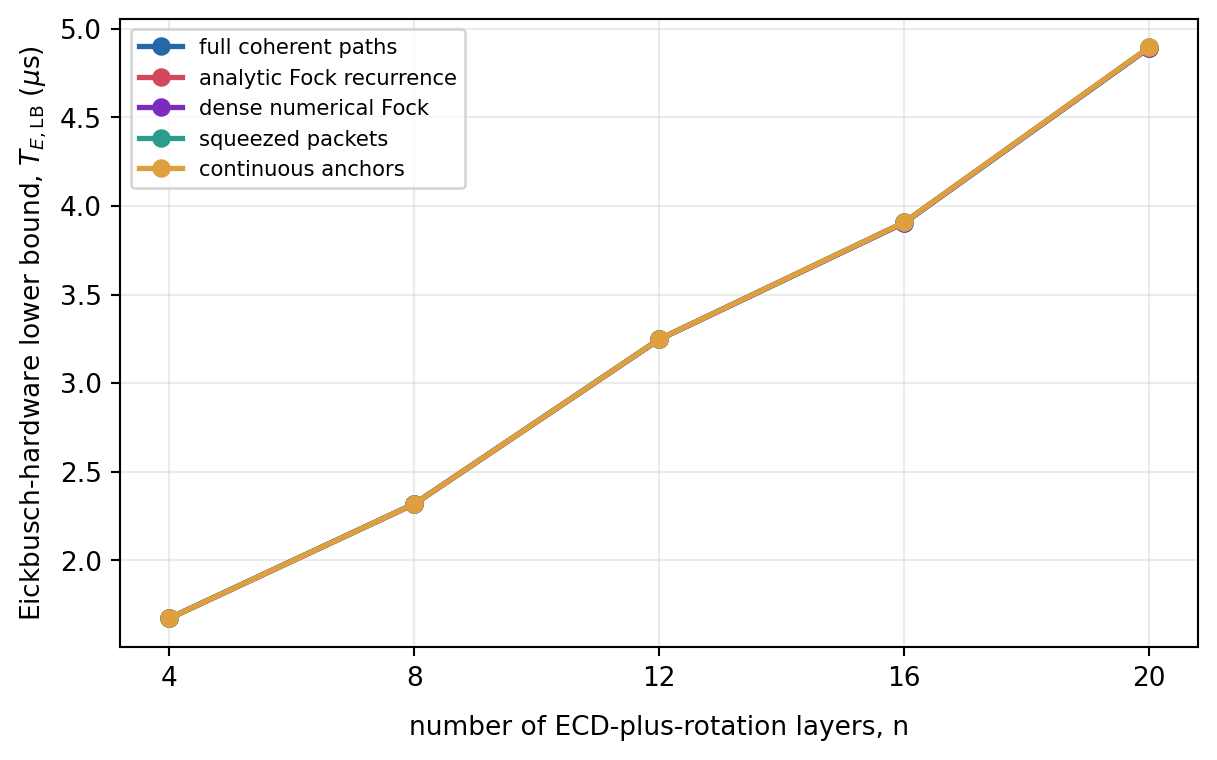
\includegraphics[width=\linewidth]{figs/gate_time_eickbusch_bound_vs_layers.png}
\end{minipage}
\caption{Requested line plots. Infidelity uses a logarithmic vertical axis.
The jump at $n=20$ combines four extra layers with a change from 1,200 to
10,000 Adam updates, so it is not a controlled depth-scaling point. At $n=20$
analytic Fock is 38.3 times faster than full coherent and 9.1 times faster than
dense numerical Fock. Physical gate times are
nearly identical because the winning displacement sequences are similar.}
\end{figure}

\textbf{Takeaway.}
At 20 layers all five methods reach $F\simeq0.998765$. Full coherent is best by
only $8.43\times10^{-9}$ over dense numerical Fock, while analytic Fock is
fastest. All five winners come from the same warm restart; a random restart remains much
worse even after 10,000 updates, showing material seed dependence. The packet
methods' bounded 64-coefficient representation is real, but their repeated
center/squeeze fits cost much more and do not improve fidelity. Both Fock methods
work well because 48 levels suffice for these sequences. Full coherent paths
retain a different advantage: the objective stays exact for displacements that
would cross a Fock boundary. These are best observed results, not
global-optimum proofs.

\newpage
\begin{figure}[p]
\centering
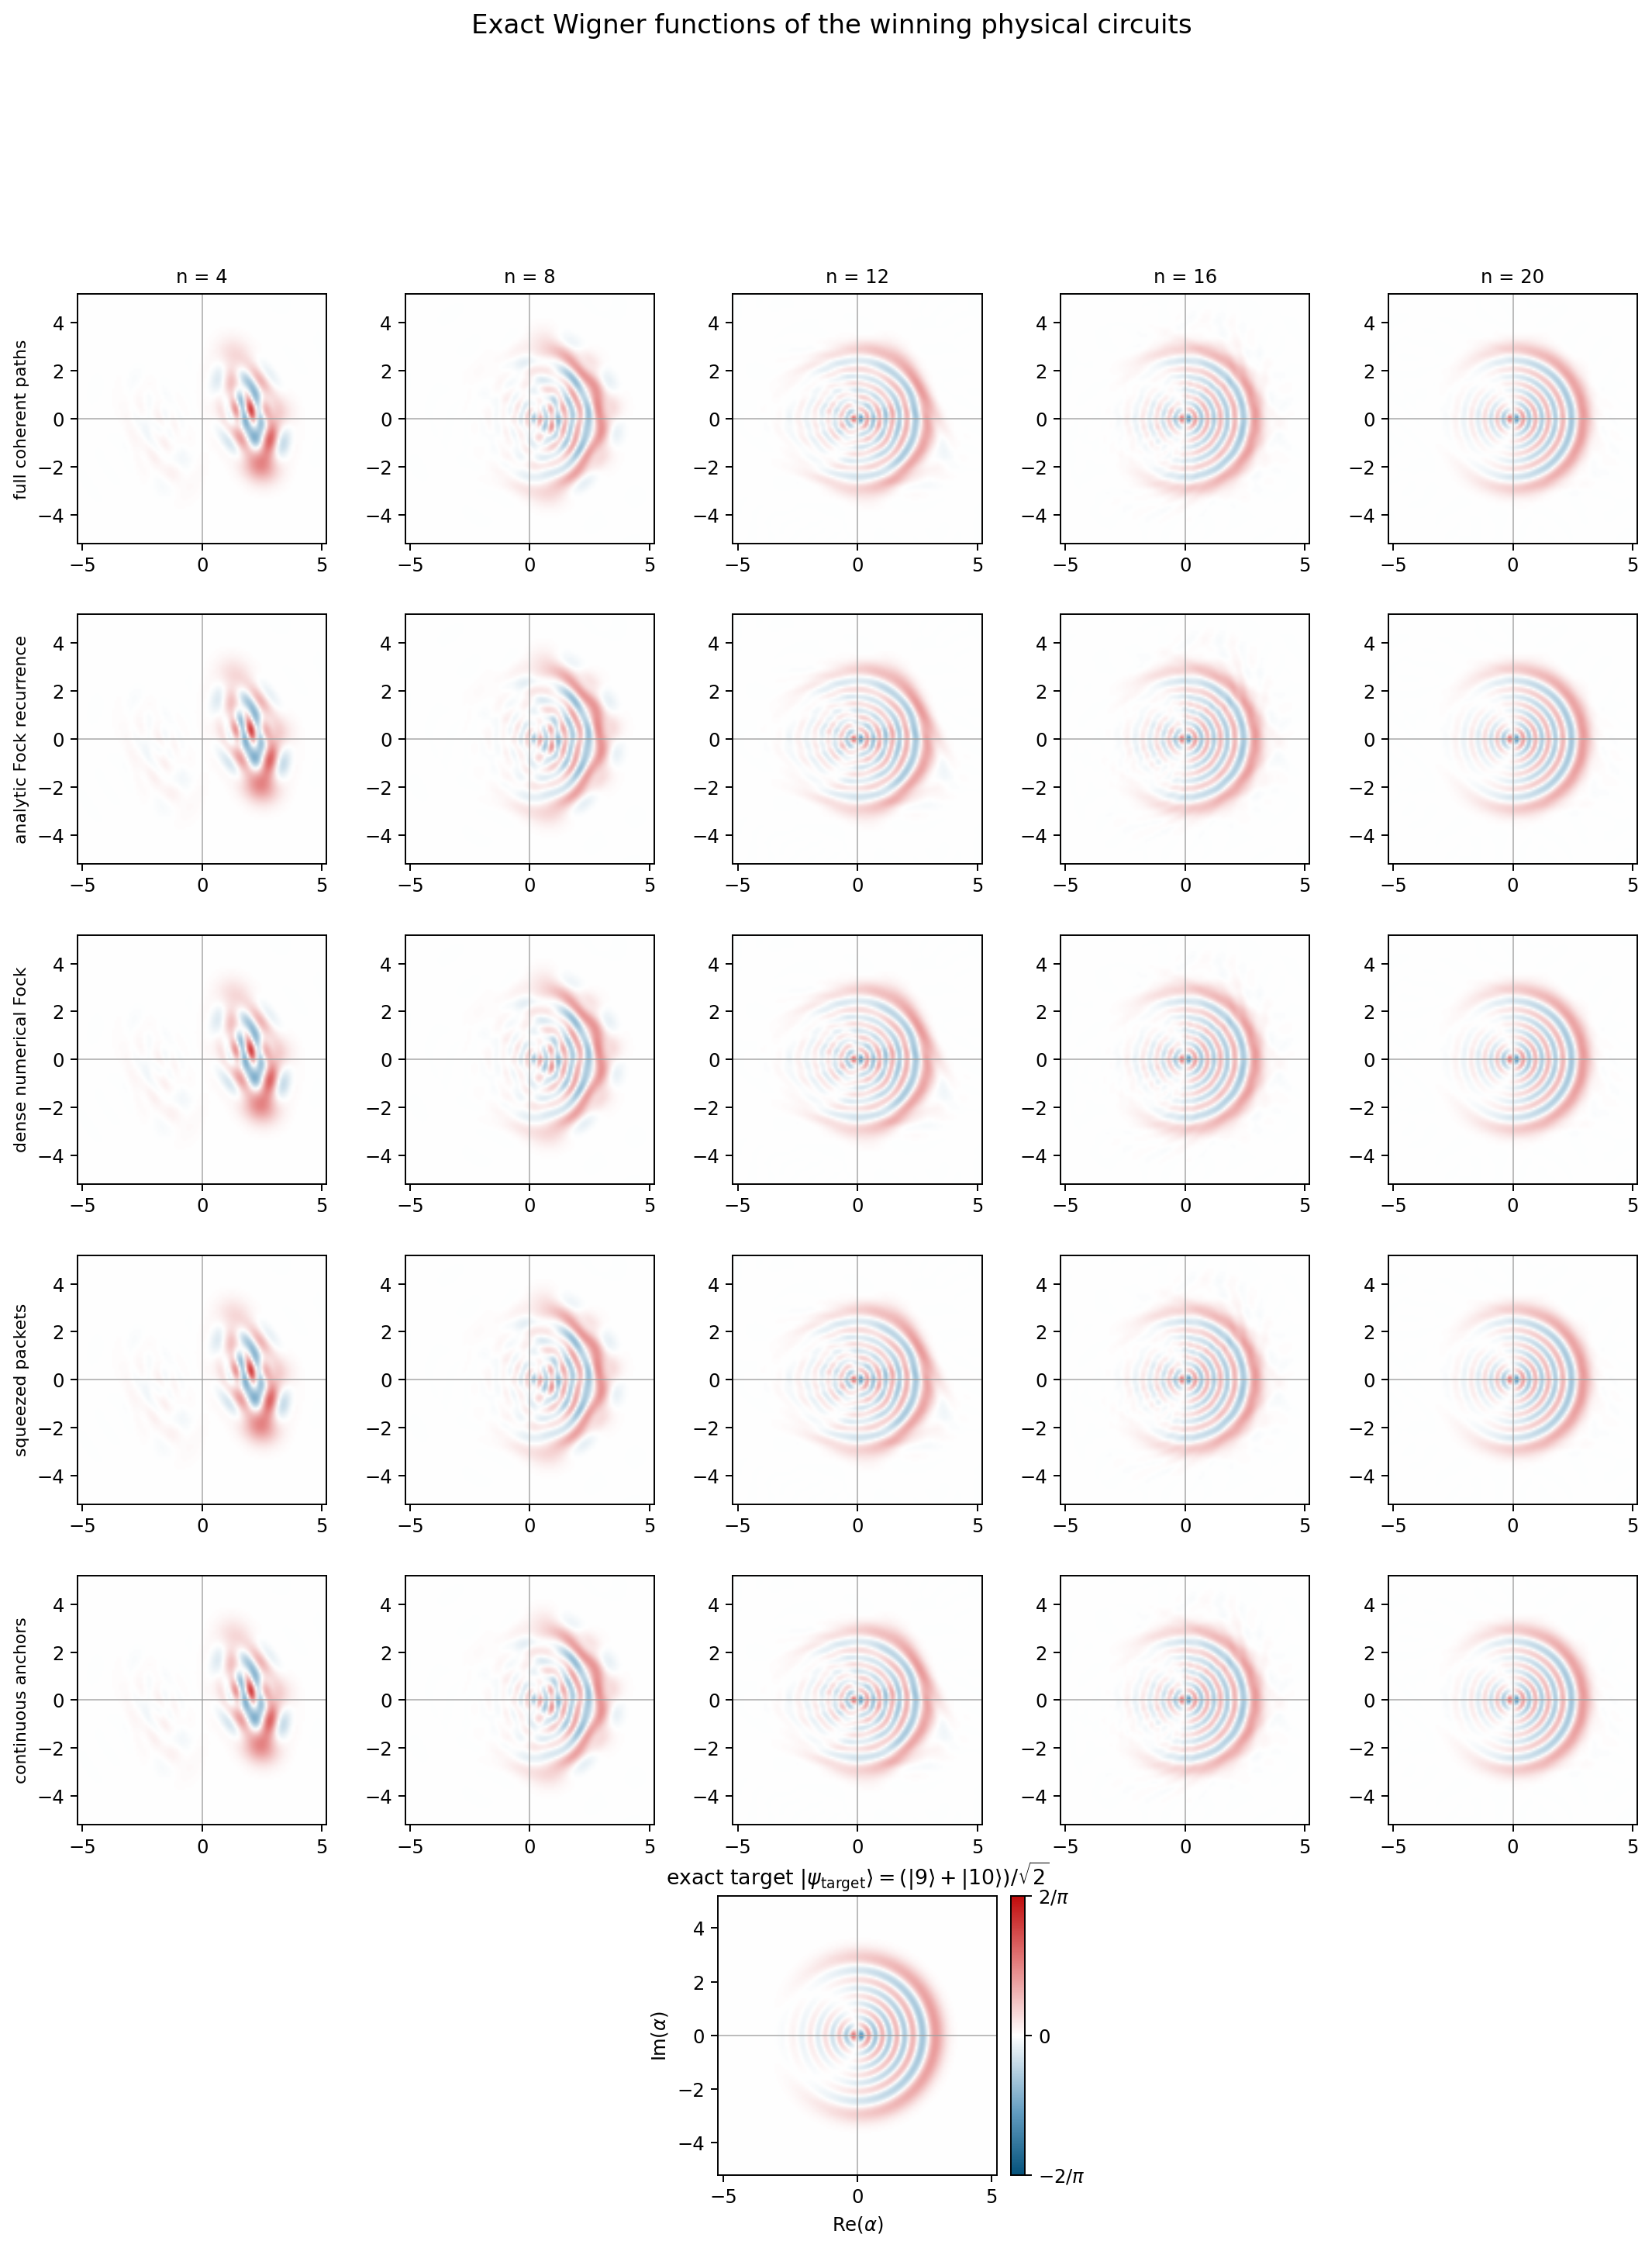
\includegraphics[width=\textwidth,height=.90\textheight,keepaspectratio]{figs/wigner_optimizer_grid.png}
\caption{Wigner functions generated with \texttt{dq.plot.wigner}. The five
columns are layer counts. Rows are full coherent, analytic Fock, dense numerical
Fock, squeezed packets, and continuous anchors. The bottom panel is the exact
target. Every optimizer panel is reconstructed from its saved exact
physical circuit and traced over the qubit; no compressed surrogate is shown.}
\end{figure}
\end{document}
